\documentclass[12pt, a4paper]{article}
\usepackage[T2A]{fontenc}
\usepackage[russian]{babel}
\usepackage[margin=0.6in]{geometry}
\usepackage{amssymb}
\usepackage{amsmath}
\usepackage{graphicx}
\usepackage{blindtext}
\usepackage[none]{hyphenat}
\usepackage[expansion=false]{microtype}
\usepackage{caption}
\usepackage{indentfirst}
\captionsetup[figure]{name=Фиг.}
\emergencystretch=3em
\def\D{\mathbb}
\graphicspath{{images/}}

\title{Математическо описание на квантовите полета}
\author{Матей Захариев}
\date{}
\begin{document}
\maketitle
{\centering\section*{15.10.2026}}
\subsection*{Класически динамични системи}
Имаме окръжност с обиколка $\Lambda$. По обиколката поставяме N на брой точки свързани с пружини. Разстоянието между тях е еднакво $\lambda = \frac{\Lambda}{N}$.
\begin{center}
	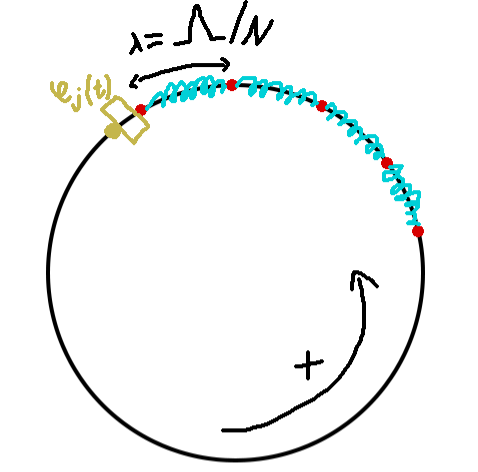
\includegraphics[scale=0.6]{circle}
\end{center}
$\varphi_j(t)$ дефинираме като отклонението на j-тото топче в момент t. По тези функции ни се дефинира система от обикновени диференциални уравнения от втори ред:
\[\ddot{\varphi_j(t)}=\kappa(\lambda-\varphi_j+\varphi_{j+1})-\kappa(\lambda-\varphi_{j-1}+\varphi_j)=\kappa(\varphi_{j+1}+\varphi_{j-1}-2\varphi_j); j\in Z_N\]

Общо за динамичните системи, при параметри $q_1$, ... $q_s$, $\ddot{q_k(t)}$ се определя от гладка функция $A_k$ на параметрите и първите производни. Съответно от Теорема на Коши, ако имаме определени стойности за параметрите и първите им производни в $t=0$, то $\exists \varepsilon>0, q_k(t), t\in(-\varepsilon,+\varepsilon)$ съществува единствено решение. Схематично се свежда до рекурсия с дълбочина 2 по следния начин. Разделяме интервала $[0,t]$ на $k(\rightarrow \infty)$ части. Дефинираме:
\[\Delta t = \frac{t}{k}, t_j=j\Delta t, q=(q_1,...q_k)\]
\[\dot{q_j}\approx\frac{(q(t_{j})-q(t_{j-1}))}{\Delta t};\ddot{q_j}\approx\frac{(\dot{q}(t_{j+1})-\dot{q}(t_j))}{\Delta t}\approx\frac{q(t_{j+1})+q(t_{j-1})-2q(t_j)}{\Delta t^2}\]
\[q(t_{j+1})=\Delta t^2A\left(q(t_j),\frac{q(t_j)-q(t_{j-1})}{\Delta t}\right)+2q(t_j)-q(t_{j-1})\]
Съответно имаме рекурсия с дълбочина 2.\\

\subsection*{Дискретна Фурие трансформация}
Имаме следното матрично представяне:
\[\xi_N:=e^{\frac{2\pi i}{N}}=cos\frac{2\pi}{N}+isin\frac{2\pi}{N}\]
\begin{center}
	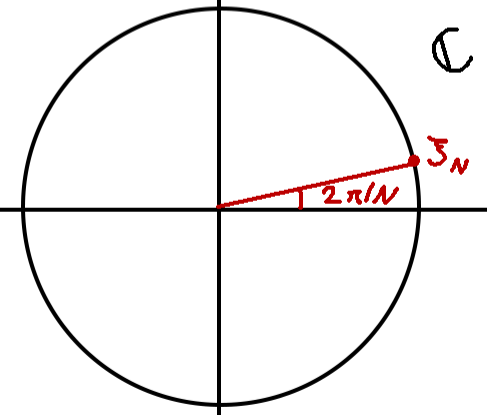
\includegraphics[scale=0.6]{complex}
\end{center}
Съответно дефиниране $U_n\in \D{C}^{NxN}$, такава че $u_{jk}=\xi^{jk}_N\frac{1}{\sqrt{N}},j,k=0,...N-1$. Тази матрица е унитарна, т.е. умножена по себе си комплексно спрегната и транспонирана дава единичната матрица. Доказателство:
\[\overline{u_jk}=\overline{\xi_N}^{jk}\frac{1}{\sqrt{N}}=\xi_N^{-jk}\frac{1}{\sqrt{N}}=v_{jk}\]
\[\sum_{k=0}^{N-1}u_{jk}v_{kl}=\sum_{k=0}^{N-1}\xi_N^{jk}\xi_N^{-kl}\frac{1}{N}=\frac{1}{N}\sum_{k=0}^{N-1}\xi_N^{k(j-l)}=
\begin{cases}
	\frac{1-\xi_N^{(j-l)N}}{1-\xi_N^{j-l}}=\frac{1-1}{1-\xi_N^{j-l}}=0;j\ne l\\
	1;j=l\\
\end{cases}
\]
Съответно имаме 2 окръжности с различни обиколки $\Lambda$ и $\tilde{\Lambda}$. Имаме N на брой $\phi$ и $\tilde{\phi}$. Съответно имаме трансформация $U_n\phi = \tilde{\phi};U_n^{-1}\tilde{\phi} = \phi$ или:
\[\phi_j = \frac{1}{\sqrt{N}}\sum_{k=0}^{N-1}e^{2\pi ijk/N}\tilde{\phi_k};\tilde{\phi_k} = \frac{1}{\sqrt{N}}\sum_{j=0}^{N-1}e^{-2\pi ijk/N}\phi_j\] 
Нека си определим $\lambda$ и $\tilde{\lambda}$ като разстоянията между точките на съответните окръжности. Дефинираме $h = \lambda\tilde\lambda N$ и $\hbar=\frac{h}{2\pi}$. Тогава за $x=j\lambda$ и $p=k\lambda$ получаваме:
\[e^{2\pi ijk/N} = e^{ixp/\hbar}

\end{document}